%! Author = joels
%! Date = 05/01/2021

\section{GUI-Design}
\subsection{Controls}
Das Aussehen von Controls wird über Attribute beeinflusst.
\subsubsection{Image}
\begin{itemize}[topsep=0pt, leftmargin=4mm]
    \setlength\itemsep{-0.3em}
    \item Bilddatei zum Projekt hinzufügen
    \begin{itemize}[topsep=0pt, leftmargin=4mm]
        \setlength\itemsep{-0.3em}
        \item Build Action: Resource
        \item Integration in Binärdatei des Projekts
    \end{itemize}
    \item Source für Dateipfad
    \begin{itemize}[topsep=0pt, leftmargin=4mm]
        \setlength\itemsep{-0.3em}
        \item Relativer Pfad beginnend bei XAML-Datei
        \item Verwendung von Ordnern möglich
    \end{itemize}
    \item Stretch für Kontrolle der Skalierung
    \begin{itemize}[topsep=0pt, leftmargin=4mm]
        \setlength\itemsep{-0.3em}
        \item Uniform: Bildverhältnis beibehalten (Standard)
        \item Fill: Fläche füllen, Bildverhältnis ignorieren
        \item UniformToFill: Fläche füllen, Bildverhältnis beibehalten
        \item None: Bild gemäss Originalgrösse darstellen
    \end{itemize}
\end{itemize}
\begin{lstlisting}
<Image Source="../Bilder/Logo.jpg" Stretch="Uniform" />
\end{lstlisting}
\subsubsection{Border}
Container für genau ein Element (Controls, oder Layouts). Verwendung zur \textcolor{blue}{Gruppierung} oder \textcolor{blue}{Hervorhebung} von Inhalten via Rahmen, Hintergrundfarbe, Runde Ecken, Sichtbarkeit
\begin{lstlisting}
<Border BorderThickness="2"
    BorderBrush="Black"
    Background="#f0f0f0">
    <StackPanel>
        <Button Content="Button 1" Margin="5" />
        <Button Content="Button 2" Margin="5" />
        <Button Content="Button 3" Margin="5" />
    </StackPanel>
</Border>
\end{lstlisting}
\subsubsection{Canvas}
2D-Zeichenfläche für einfache geometrische Objekte (Shapes). Absolute Positionierung in X/Y-Raster (Keine Layout-Logik. Kind-Elemente erhalten Attached Porperties)\\
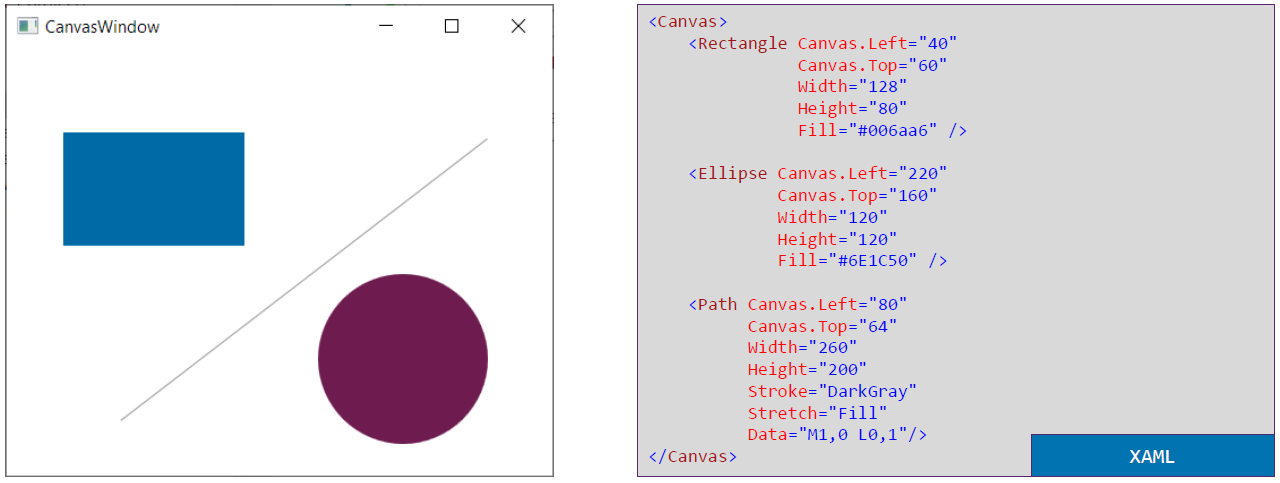
\includegraphics{canvas.png}
\subsubsection{Window Clipping}
Die Form eines Window kann mittels Clipping beliebig verändert werden. Das Window muss dazu jedoch korrekte Einstellungen haben:
\begin{lstlisting}
<Window AllowsTransparency="True"
        WindowStyle="None"
        Width="400"
        Height="200"
        Background="#6E1C50">

    <Window.Clip>
        <RectangleGeometry RadiusX="30"
                           RadiusY="30"
                           Rect="0,0,400,200" />
    </Window.Clip>
    <Grid>
        <Label Content="Clipped Window"
               HorizontalAlignment="Center"
               VerticalAlignment="Center"
               Foreground="White" />
    </Grid>
</Window>
\end{lstlisting}
\subsection{Resources}
Beliebige Objekte, die in XAML definiert werden können: Brush, Color, String.\\
Resourcen besitzten eine eindeutige Identifikation. Zuweisung des XAML-Attributs mit \textcolor{blue}{x:key}. Dies erlaubt später eine Referenzierung.
\subsubsection{Resource Directory}
\begin{itemize}[topsep=0pt, leftmargin=4mm]
    \setlength\itemsep{-0.3em}
    \item Container zur Speicherung von Resources
    \item Zugriff über Schlüssel der Resource (x:Key)
    \item Teil aller FrameworkElement-Ableitungen (Zugriff über Property Element Syntax)
    \item Beispiele:
    \begin{itemize}[topsep=0pt, leftmargin=4mm]
        \setlength\itemsep{-0.3em}
        \item Application.Resources
        \item Window.Resources
        \item Button.Resources
        \item Label.Resources
    \end{itemize}
\end{itemize}
\subsubsection{Verwendung von Resources}
\textbf{Ziel:} Objekte zentral definieren und n-fach wiederverwenden
\begin{lstlisting}
// XAML
<Window>
  <Window.Resources>
    <SolidColorBrush x:Key="OSTBrush" Color="#6E1C50" />
  </Window.Resources>
  <StackPanel>
    <Label Content="Variante 1" Foreground="White">
      // Property Element Syntax
      <Label.Background>
        <StaticResource ResourceKey="OSTBrush" />
      </Label.Background>
    </Label>
    <Label Content="Variante 2"
           Foreground="White"
           // Attribute Syntax mit Markup Extension
           Background="{StaticResource ResourceKey=OSTBrush}" />
    <Label Content="Variante 3"
           Foreground="White"
           // Attribute Syntax mit Markup Extension
           Background="{StaticResource OSTBrush}" />
  </StackPanel>
</Window>

// C#
// via FrameworkElement.FindResource( ... )
var brush = FindResource("OSTBrush") as Brush;
\end{lstlisting}
\subsubsection{Auflösung von Resources}
Suchreihenfolge (bricht beim ersten Treffer ab):\\
\textbf{1.} Aktuelles Element und alle Parent-Elemente\\
\textbf{2.} In \textcolor{blue}{Application.Resources}\\
\textbf{3.} In System-Ressourcen\\
\subsubsection{Statische und dynamische Ressourcen}
\textbf{\textcolor{blue}{Statische Resources:}}
\begin{itemize}[topsep=0pt, leftmargin=4mm]
    \setlength\itemsep{-0.3em}
    \item Einmalige Auswertung der Resource
    \item Auswertung bei Kompilierung
    \item Unveränderlich zur Laufzeit
    \item Extension: $\{$StaticResource Key$\}$
\end{itemize}
\textbf{\textcolor{blue}{Dynamische Resources:}}
\begin{itemize}[topsep=0pt, leftmargin=4mm]
    \setlength\itemsep{-0.3em}
    \item Mehrfache Auswertung der Resource
    \item Auswertung bei Ausführung
    \item Veränderlich zur Laufzeit
    \item Extension: $\{$DynamicResource Key$\}$
\end{itemize}
\begin{lstlisting}
// XAML
<Window>
  <Window.Resources>
    <SolidColorBrush x:Key="OSTBrush" Color="#6E1C50" />
  </Window.Resources>
  <StackPanel>
    <Label Content="OK"
           Foreground="White"
           Background="{DynamicResource OSTBrush}" />
    <Button Content="Update"
            Click="UpdateResource" />
  </StackPanel>
</Window>

// Code Behind
private void UpdateResource(object sender, RoutedEventArgs e) {
    Resources["OSTBrush"] = new SolidColorBrush(Colors.Blue);
}
\end{lstlisting}
\subsubsection{Beliebige Typen}
Ein Resource Dictionary nimmt alle Elemente auf, die in XAML definierbar sind. Aufig werden Basistypen benötigt wie strings, Zahlen, etc.
\begin{lstlisting}
// Stystem.Runtime enthält Basistypen
<Window xmlns:s="clr-namespace:System;assembly=System.Runtime">
  <Window.Resources>
    <s:Double x:Key="MarginVertical">2</s:Double>
    <s:Double x:Key="MarginHorizontal">5</s:Double>
    <Thickness x:Key="Margin"
        Top="{StaticResource MarginVertical}"
        Bottom="{StaticResource MarginVertical}"
        Left="{StaticResource MarginHorizontal}"
        Right="{StaticResource MarginHorizontal}" />
  </Window.Resources>
</Window>
\end{lstlisting}
\subsubsection{Zugriff auf CLR-Werte}
Gelegentlich ist es nötig, auf statische Werte der CLR zuzugreifen. Zugriff via Markup Extension: \textcolor{blue}{x:Static}. Keine WPF-Resources. Werte definiert in normalen Klassen.
\begin{lstlisting}
// C#
public static class MyRes {
    public static SolidColorBrush OSTBrush = new SolidColorBrush(Color.FromRgb(110, 28, 80));
}

// XAML
<Label Content="x:Static"
   Background="{x:Static local:MyRes.OSTBrush}"
   Foreground="{x:Static SystemColors.ControlLightBrush}"
   FontFamily="{x:Static SystemFonts.CaptionFontFamily}"
   FontSize="{x:Static SystemFonts.CaptionFontSize}" />
\end{lstlisting}
\subsubsection{Eigenständige Resource Dictionaries}
In separater .xaml-Datei mit XML-Root $<$ResourceDictionary$>$. In andere Dictionaries als Merged Dictionary integrierbar.
\begin{lstlisting}
// MyDictionary.xaml
<ResourceDictionary>
  <SolidColorBrush x:Key="OSTBrush2" Color="#6E1C50" />
</ResourceDictionary>
// MainWindow.xmal
<Window>
  <Window.Resources>
    // Für Merges zwingend, sonst optional
    <ResourceDictionary>
      <SolidColorBrush x:Key="OSTBrush" Color="#6E1C50" />
      <ResourceDictionary.MergedDictionaries>
        <ResourceDictionary Source="MyDictionary.xaml"/>
      </ResourceDictionary.MergedDictionaries>
    </ResourceDictionary>
  </Window.Resources>
  <Label Content="Externe Resource"
    Foreground="White"
    Background="{StaticResource OSTBrush2}" />
</Window>
\end{lstlisting}
\subsubsection{Externe Resources}
Dictionaries können via Pack URI aus anderen Assemblies eingebunden werden.

\subsection{Styles}
Resources können mehrfach verwendet werden, müssen aber bei jedem Element referenzieren. Das gibt Duplizierten Code.
\subsubsection{Explizite Styles}
\begin{lstlisting}
<Window>
  <Window.Resources>
    // Mit oder ohne TargetType
    <Style x:Key="MyButtonStyle" TargetType="Button">
      <Setter Property="Background" Value="Blue" />
      <Setter Property="Foreground" Value="Black" />
      <Setter Property="BorderBrush" Value="Black" />
      <Setter Property="BorderThickness" Value="1" />
    </Style>
  </Window.Resources>
  <StackPanel>
    <Button Style="{StaticResource MyButtonStyle}"
        Content="OK" />
    <Button Style="{StaticResource MyButtonStyle}"
        Content="Cancel" />
  </StackPanel>
</Window>
\end{lstlisting}
\subsubsection{Implizite Styles}
Ohne Key wirkt der Style für alle Controls des angegeben Typs.
\begin{lstlisting}
<Window>
  <Window.Resources>
    <Style TargetType="Button"> // Style erhält automatisch den key x:key="{x:Type Button}"
      <Setter Property="Background" Value="Blue" />
      <Setter Property="Foreground" Value="Black" />
      <Setter Property="BorderBrush" Value="Black" />
      <Setter Property="BorderThickness" Value="1" />
    </Style>
  </Window.Resources>
  <StackPanel>
    // Keine Style Attribute mehr nötig
    <Button Content="OK" />
    <Button Content="Cancel" />
  </StackPanel>
</Window>
\end{lstlisting}
\subsubsection{Styles erweitern}
Styles sind mit Inline-Attributen kombinierbar (eignet sich für einmalige Anpassungen). Styles können auch vererbt werden. $\rightarrow$ Kann Umfang der Ressourcen reduzieren
\begin{lstlisting}
// Mit Inline Attribute
<Button Style="{StaticResource NormalButton}"
    Background="Red"
    Content="Cancel" />

// Vererbung
<Window.Resources>
  <Style x:Key="NormalButton" TargetType="Button">
    ...
  </Style>
  <Style x:Key="DangerButton"
      BasedOn="{StaticResource NormalButton}"
      TargetType="Button">
    <Setter Property="Background" Value="Red" />
  </Style>
</Window.Resources>
...
<Button Style="{StaticResource DangerButton}"
    Content="Cancel" />
\end{lstlisting}
\subsubsection{Komplexe Werte}
Können über setzten des Value-Attributs auf dem Setter Element verwendet werden. Beispiel eines Gradient Hintergrund:
\begin{lstlisting}
<Window.Resources>
  <Style x:Key="BrushButton" TargetType="Button">
    <Setter Property="Background">
      <Setter.Value>
        <LinearGradientBrush StartPoint="0,0" EndPoint="0,1">
          <GradientStop Offset="0" Color="Red" />
          <GradientStop Offset="0.5" Color="Yellow" />
          <GradientStop Offset="1" Color="Red" />
        </LinearGradientBrush>
      </Setter.Value>
    </Setter>
  </Style>
</Window.Resources>
<Button Style="{StaticResource BrushButton}" Content="Brush" />
\end{lstlisting}
\subsubsection{Trigger}
Trigger erlauben Stylings basierend auf dem Zustand eines Elementes. Beliebige Attribute des Elements sind auswertbar. Beispiel: Veränderung des Cursors abhängig vom Button-Label:
\begin{lstlisting}
<Window.Resources>
  <Style x:Key="TriggerButton" TargetType="Button">
    <Style.Triggers>
      <Trigger Property="Content" Value="Link">
        <Setter Property="Cursor" Value="Hand" />
      </Trigger>
      <Trigger Property="Content" Value="Edit">
        <Setter Property="Cursor" Value="Pen" />
      </Trigger>
    </Style.Triggers>
  </Style>
</Window.Resources>
<Button Style="{StaticResource TriggerButton}" Content="Link" />
<Button Style="{StaticResource TriggerButton}" Content="Edit" />
\end{lstlisting}
\subsubsection{Themes}
WPF hat kein Themes-Konzept. Kann aber nachgebaut werden:\\
Dazu gleiche x:Key styles in mehreren Resource Dictionaries definieren. Laden des gwünschten Dictionary zur Laufzeit und Zuweisung der Styles über DynamicResource.
\subsection{Control Templates}
\begin{itemize}[topsep=0pt, leftmargin=4mm]
    \setlength\itemsep{-0.3em}
    \item Control Templates beschreiben die visuelle Repräsentation von XAML-Controls (Elemente, die im Visual tree eingefügt werden)
    \item Der Zugriff auf das aktuelle Template erfolgt über das Attribut \textcolor{blue}{Control.Template}
    \item Eigene Control Templates: Option1: Als ControlTemplate-Resource. Option2: Innerhalb eines Styles
\end{itemize}
\textbf{\textcolor{blue}{ContentPresenter:}}\\
Platzhalter für den Content des Elements\\
\textbf{\textcolor{blue}{TemplateBinding:}}\\
Markup Extension für das Binding an Attribute. Nur in Control Templates verwendbar.
\subsection{Guidelines}
Keine expliziten, bzw. ernstzunehmenden Guidelines für WPF verfügbar. Empfehlung: Guidelines und Libraries
nutzen, die sich andernorts bewährt haben. z.B. Material Design in XAML, MahApps.Metro
\pagebreak